\documentclass[a4paper]{article}
\title{\Huge{\textsc{Evolutionary Algorithms for Iterated Prisoner's Dilemma}}}
\usepackage[margin=3cm]{geometry}
\usepackage{graphicx}
\usepackage{wrapfig}
\usepackage{caption}
\usepackage{amsmath}
\usepackage{subcaption}
\usepackage[export]{adjustbox}
\usepackage{enumerate}
\usepackage{url}
\usepackage{authblk}
\usepackage{float}
\usepackage{wrapfig}
\usepackage{setspace}
\usepackage{mdframed}
\usepackage{booktabs}
\usepackage{ragged2e}

\def\changemargin#1#2{\list{}{\rightmargin#2\leftmargin#1}\item[]}
\let\endchangemargin=\endlist 

\DeclareMathSizes{10}{10}{10}{10}
\begin{document}

    \newgeometry{left=4cm,right=4cm,top=4cm,bottom=6cm}
	\begin{titlepage}
	    \begin{center}
	        \vspace*{1cm}
	        
	        {\huge{\textsc{Evolutionary Algorithms for Iterated Prisoner's Dilemma}}\\}
	        \vspace{8mm}
	        {\large{Nishant Rai}}\\
			\vspace{3mm}
			
			{\normalsize{Department of Computer Science and engineering\\}}
	        \vspace{4mm}
        	\vspace{7mm}
	        \textbf{Abstract\\}
        	\vspace{4mm}
        	\noindent
{\justifying{The project deals with the problem of computing successful strategies for Iterated Prisoner's dilemma. We propose multiple algorithms to compute good strategies which perform well against a set of baseline algorithms (Including the extremely simple yet effective 'Tit for Tat'). We discuss Axelrod's Tournament and use a similar setup to decide the effectiveness of the computed strategies. The result section shows the superiority of the strategies computed using them.} \par}
			\vfill
			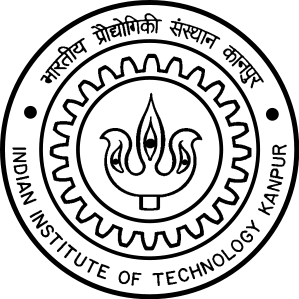
\includegraphics[width=0.25\textwidth]{iitklogo.png}\\[0.1in]
            \vspace{3mm}
            \normalsize{Under the guidance of Dr. Vimal Kumar\\}
            \vspace{1mm}
            {Indian Institute of Technology, Kanpur}
	    \end{center}
	\end{titlepage}
	\restoregeometry

	\tableofcontents
	
	\pagebreak	
	
	\section{Introduction}
	
	The Prisoner's Dilemma is a classic problem in game theory, discovered in 1950 by Melvin Dresher and Merrill Flood, whose purpose is, among other things, to describe a situation in which rational behavior (defined as that behavior which will maximize one's expected benefit) can be, in a sense, self-undermining. It has become a popular problem because it is seen as fundamentally similar to real-world problems in sociology and politics. \\
	The Prisoner's Dilemma can be described as follows: suppose that two individuals, A and B, have been arrested in connection with a crime. Each is put in a separate interview room and told that a deal may be available to them depending on whether each provides testimony against the other (defects) or keeps silent (cooperates). Each individual is assumed to want to do as well as possible for themselves without regard to the welfare of the other player.\\

	\begin{table}[H]
	\centering
	\begin{tabular}{|c|c|c|}
	\hline
						& B co-operates            & B defects 					\\ \hline
	A co-operates  		& (R,R) 		 			& (S,T)         			\\ \hline
	A defects 			& (T,S)           			& (P,P)            			\\ \hline
	\end{tabular}
	\caption{Payoff matrix for the Prisoner's Dilemma}
	\end{table}
		
	This situation is formally specified by the matrix in Figure 1, subject to the following definitions and restrictions:
	\begin{itemize}
		\item T : \textbf{Temptation} for unilateral defection
		\item R: \textbf{Reward} for mutual cooperation
		\item P : \textbf{Punishment} for mutual defection
		\item S: \textbf{Sacrifice} for unilateral cooperation	
	\end{itemize}
	
	A variant of the classical prisoner's game arises as a result of repeated games. It is termed as Iterated Prisoner's Dilemma. The situation is more interesting when the game satisfies the following conditions,
	\begin{enumerate}
	\item The number of moves should not be known to the two players.
	\item The winner is the player with the highest score in the end.
	\item Usually, there are many players in the fray, and there is a Round Robin Tournament among all the players - the player with the highest score wins.		
	\end{enumerate}
	
	\section{Related Work}
	
	\section{Axelrod's Tournament}

	In 1980, Robert Axelrod, professor of political science at the University of Michigan, held a tournament of various strategies for the prisoner's dilemma. He invited a number of well-known game theorists to submit strategies to be run by computers. In the tournament, programs played games against each other and themselves repeatedly. Each strategy specified whether to cooperate or defect based on the previous moves of both the strategy and its opponent.\\
	Some of the strategies submitted were:
	\begin{itemize}
	\item \textbf{Always Defect}: This strategy defects on every turn. This is what game theory advocates. It is the safest strategy since it cannot be taken advantage of. However, it misses the chance to gain larger payoffs by cooperating with an opponent who is ready to cooperate.
	\item \textbf{Always Cooperate:} This strategy does very well when matched against itself. However, if the opponent chooses to defect, then this strategy will do badly.
	\item \textbf{Random:} The strategy selects its move randomly i.e. cooperates and defects 50\% of the time.
	\end{itemize}
	
	All of these strategies are prescribed in advance. Therefore, they cannot take advantage of knowing the opponent's previous moves and figuring out its strategy. The winner of Axelrod's tournament was the 'Tit for Tat' strategy. The strategy cooperates on the first move, and then does whatever its opponent has done on the previous move. Thus, when matched against the all-defect strategy, 'Tit for Tat' strategy always defects after the first move. When matched against the all-cooperate strategy, 'Tit for Tat' always cooperates. This strategy has the benefit of both cooperating with a friendly opponent, getting the full benefits of cooperation, and of defecting when matched against an opponent who defects. When matched against itself, the 'Tit for Tat' strategy always cooperates.\\
	'Tit for Tat' relies on the assumption that its opponent is trying to maximize his score. When paired with a mindless strategy like 'Random', 'Tit for Tat' sinks to its opponent's level. For that reason, 'Tit for Tat' cannot be called a 'best' strategy. It must be realized that there really is no 'best' strategy for prisoner's dilemma. Each individual strategy will work best when matched against a 'worse' strategy. In order to win, a player must figure out his opponent's strategy and then pick a strategy that is best suited for the situation.
	
	\subsection{Features of Successful Strategies}

A strategy (pure) for a player in a particular game is a plan describing what move that player should take in each possible situation (information state) that might arise for him.
In Axelrod’s IPD tournaments, strategies exhibiting the following four properties tended to be more successful (i.e., to accumulate higher total payoffs), with the clear-cut winner being the Tit-for-Tat strategy.
	\begin{itemize}
		\item \textbf{Niceness}: Never be the first to defect.
		\item \textbf{Provocability}: Get mad quickly at defectors and retaliate.
		\item \textbf{Forgiveness}: Do not hold a grudge once you have vented your anger.
		\item \textbf{Clarity}: Act in ways that are straightforward for others to understand.
	\end{itemize}

	\subsection{Axelrod Strategies}	

As we have seen earlier that 'Tit for Tat', such a simple strategy turned out to be the winner in Axelrod's tournament. Axelrod set out to find other simple strategies with similar or greater power.\\
Axelrod adopted a simple but elegant way for encoding strategies, and then used a single-objective evolutionary algorithm to obtain optimal strategies. His encoding scheme remained a standard way of handling the IPD problem and is described below. We also adopt a similar encoding scheme to compute optimal strategies for the game. Axelrod's method had the following features,
	\begin{itemize}
	\item The next move depends upon the behavior of both the parties during previous three (In general k, termed as memory length in this paper) moves.
	\item We have four possibilities for the previous move, which are as follows,
	\begin{itemize}
		\item CC or R for Reward
		\item CD or S for Sucker
		\item DC or T for Temptation
		\item DD or P for Penalty
	\end{itemize}		
	\item We code the particular behavioral sequence as a 3-letter string.	
	\item We then use the 3-letter sequence to generated a number between 0 and 63 (i.e. $4^{3} = 4^{k}$) by interpreting it as an integer base 4 (Since there were 4 possibilities for each turn).
	\item Strategy string : 64-bit binary string of C's and D's where he $i^{th}$ bit corresponds to the $i^{th}$ behavioral sequence.
	\end{itemize}

	The following \textbf{critical} points should be observed,
	\begin{itemize}
	\item The behavior of the player is undefined in the first three moves of the game (Since we do not have histories of the game).
	\item We also add six bits to the encoding to specify a strategy's premises, i.e. assumption about the pre-game behavior.
	\item Together, each of the 70-bit strings represent a particular strategy (i.e. State-action codes)	
	\end{itemize}		
	
	\section{Motivation}
	
	\section{Proposed Algorithms}
	
	\subsection{Axelrod Strategies using Evolutionary Algorithms}

	\subsection{Reinforcement Learning for Adaptive Strategies}
	
	\section{Experiments}
	
	\subsection{Tournament Setup}
	
	\subsection{Baseline Strategies}

	\section{Results}
	
	\section{Observations}
	
	\subsection{Effect of Memory on Strategies}	
		
	\section{Future Work}
			
\end{document}


